\section{A finite laboratory}\label{sec:lab}

We now illustrate each part of the chain in Figure~\ref{fig:overview} on finite Markov chains. The point is not to discover the theorems of Sections~\ref{sec:duality} and~\ref{sec:audits} empirically, since they need no such support. It is to show them operating on concrete substrates, to check the numerical pipeline against them, and to isolate the effects that depend on the chosen example rather than on a theorem.

\subsection{Substrates, lenses, and protocol}\label{sec:lab-setup}

\paragraph{Module-ring chain.} The main substrate has \(M=6\) rings of \(L=10\) states, \(60\) states in all. On ring \(m\) each state sends weight \(e^{+A_m/(2L)}\) clockwise and \(e^{-A_m/(2L)}\) counter-clockwise, and neighbouring rings are joined at their first state by a symmetric bridge of weight \(0.2\); rows are then normalized. Row normalization adds only a gradient to the edge log-ratios, so each ring carries cycle affinity exactly \(A_m\). We use \(A_m\) evenly spaced from \(1.0\) to \(-0.5\). Every edge is bidirectional, so all path audits of the true chain are finite. Trajectories start from the uniform law.

\paragraph{Ladder chain.} For the resolution ladder we use the same rings joined by \emph{two} bridges per neighbouring pair, at positions \(0\) and \(L/2\), again with weight \(0.2\).

\paragraph{Lenses.} A lens is a partition \(f:Z\to X\) of the states into blocks. To audit observed trajectories we apply \(f\) pointwise to each sampled path. When a Markov kernel at the coarse level is needed, as for the ladder, we use stationary-conditional lumping \cite{kemeny1960finite,buchholz1994lumpability},
\[
Q_{ab}=\sum_{i:f(i)=a}\pi(i\mid a)\sum_{j:f(j)=b}P_{ij},
\]
where \(\pi\) is the stationary law of \(P\). The lumped kernel summarizes the coarse support structure. It is not used for any data-processing claim, because the lumped chain is generally not the law of the observed paths.

\paragraph{Protocol.} Every design choice (substrate, partition seed, proxy permutation, sample sizes, regularization) is fixed before running, and every run is reported. The five ``seeds'' mean different things in different experiments. For the path audit and the proxy comparison they are independent samples from one fixed design. For the price curve each seed also draws its own random partition and estimates its own cost. The ladder computation is deterministic, so its seed labels are repetitions. All numbers below come from the receipts listed in Appendix~\ref{app:repro}.

\subsection{Coarse observation never inflates the audit}\label{sec:lab-dpi}

We sample \(N=2000\) trajectories of length \(80\) from the module-ring chain and compute the reversal-mixture audit \(\Sigma_{5,\varepsilon}\) (windows of six states, \(\varepsilon=0.01\)) on the micro paths and on the same paths observed through \(k\in\{2,4,8,16,32\}\) contiguous blocks.

The micro audit is \(0.0330\pm0.0017\) (mean \(\pm\) s.d.\ over five seeds). The observed audit rises with resolution, from \(1.5\times10^{-4}\) at \(k=2\) to \(0.0293\) at \(k=32\), and stays below the micro audit in every seed, with the smallest mean margin \(0.00372\) at \(k=32\) (Figure~\ref{fig:dpi}). Proposition~\ref{prop:mixture} guarantees this on every sample, so the result is a consistency check of the implementation, not an independent discovery. It also shows the other half of the story: coarse observation can hide most of the drive, since at \(k=2\) almost none is visible.

The raw micro empirical audits are infinite in every seed: some micro windows were never seen reversed, with mean missing-reverse mass \(0.00205\). Raw observed audits are infinite whenever their missing-reverse mass is positive; its mean over seeds falls from \(0.00145\) at \(k=32\) to \(2.3\times10^{-5}\) at \(k=2\). These are sampling gaps, not one-way edges, since the true chain is fully bidirectional. They are exactly why the regularized audit is needed for a finite comparison.

\begin{figure}[tbp]
\centering
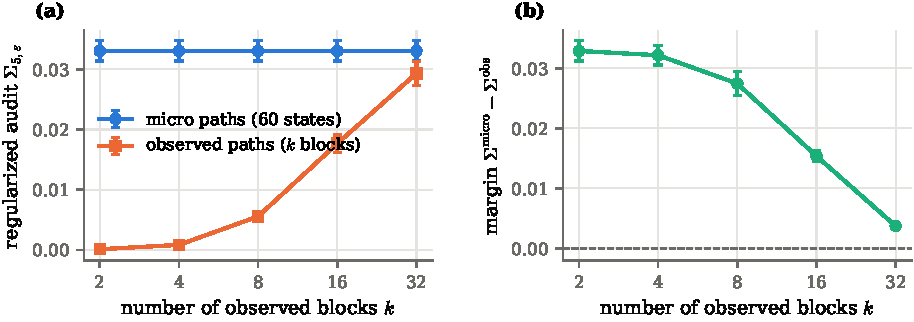
\includegraphics[width=\linewidth]{figures/fig_dpi_audit.pdf}
\caption{Coarse observation hides directionality but never creates it. (a)~Reversal-mixture path audit \(\Sigma_{5,\varepsilon}\) (\(\varepsilon=0.01\)) of micro trajectories and of the same trajectories observed through \(k\) contiguous blocks. (b)~Margin between the two. Points are means over five independent samples; bars are standard deviations. The margin is nonnegative on every sample by Proposition~\ref{prop:mixture}.}
\label{fig:dpi}
\end{figure}

\subsection{The price of an inherited budget}\label{sec:lab-price}

\paragraph{Cost.} We partition the module-ring chain into \(k=8\) random blocks, sample \(8000\) trajectories of length \(80\), and give each micro transition the cost \(\max\{0,\log(P_{ij}/P_{ji})\}\). The macro cost \(u_{ab}\) is the average of this cost over observed transitions from block \(a\) to block \(b\), shrunk toward the global mean by one pseudo-observation so that unobserved macro transitions have a defined cost.

This ledger is a modelling choice, and it should not be confused with entropy production. The log-ratio of a single edge depends on how the rows are normalized: it changes by a gradient \(\phi_j-\phi_i\) under a change of state potentials, and only its sums around cycles are invariant. The stationary entropy production instead uses \(\log[\pi_iP_{ij}/(\pi_jP_{ji})]\). Moreover, the macro Gibbs array has full support and may place mass on block transitions that the micro chain never makes. The experiment is therefore a synthetic closure on an estimated cost array; it does not construct micro maintenance protocols for each macro transition.

\paragraph{Sweep.} With uniform row weights, we solve the budget problem of Theorem~\ref{thm:duality} for \(25\) budgets \(b=\cmin+\alpha(c_0-\cmin)\), with \(\alpha\) evenly spaced from \(0.05\) to \(1.10\). Figure~\ref{fig:budget} shows the result. The price falls from \(160.9\pm15.9\) at \(\alpha=0.05\) to \(0.90\pm0.35\) at \(\alpha=0.969\), and is exactly zero for the three budgets with \(\alpha>1\) in all five seeds. In the active region the solver meets the budget to within \(3\times10^{-13}\) in every seed. In the slack region the achieved cost stays at \(c_0\), below the budget. The per-seed Spearman correlation between budget and price is \(-0.99923\); it differs from \(-1\) only because the three slack prices are tied at zero.

All of this is predicted by Proposition~\ref{prop:regimes}: a strictly decreasing price on \((\cmin,c_0)\), divergence as \(b\to\cmin\), and zero price above \(c_0\). The experiment adds no evidence for the shape of the curve. What it shows is that a cost read off a lower-layer ledger gives a nondegenerate price at the next layer. The cost is nonconstant within rows, so the price is identifiable, and the curve spans two orders of magnitude before it vanishes.

\begin{figure}[tbp]
\centering
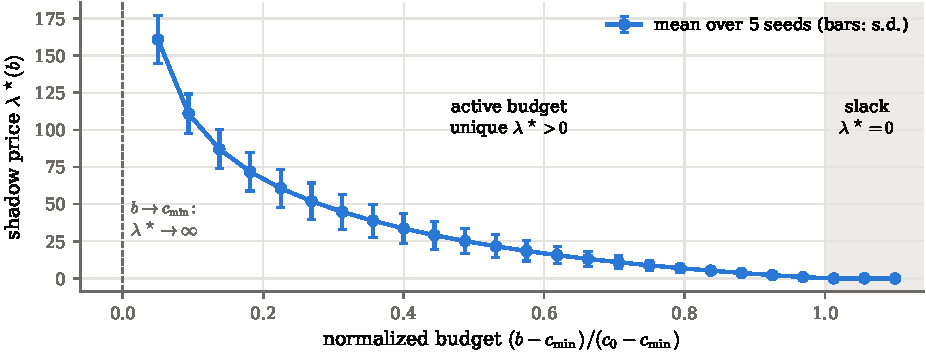
\includegraphics[width=\linewidth]{figures/fig_budget_price.pdf}
\caption{Shadow price of an inherited budget. The horizontal axis is the budget normalized so that \(0\) is the cheapest feasible cost \(\cmin\) and \(1\) is the cost \(c_0\) of the unconstrained (uniform) closure. Points are means over five seeds, each with its own random partition and estimated cost; bars are standard deviations. Shading marks the slack regime, where the price is exactly zero.}
\label{fig:budget}
\end{figure}

\subsection{Resolution adds loop directions, not necessarily drive}\label{sec:lab-ladder}

On the ladder chain we compare three lenses: whole rings (\(k=6\)), half-rings (\(k=12\)), and single states (\(k=60\)). For each, we form the lumped kernel, its bidirectional support graph, a cycle basis, and the cycle affinities.

\begin{proposition}[Ladder cycle ranks]\label{prop:ladder}
For \(M\) rings of even length \(L\ge4\) with positive bridges at positions \(0\) and \(L/2\), the three support graphs have cycle ranks \(0\), \(M-1\), and \(2M-1\).
\end{proposition}

For \(M=6\) this gives \(0,5,11\), which is what the code reports. The construction is deterministic, so the five seed labels repeat a single computation rather than test robustness. The proof is a count of edges (Appendix~\ref{app:proofs}).

These are the dimensions of the \emph{available} cycle coordinates. The dimension actually \emph{driven} is smaller (Figure~\ref{fig:ladder}). The model has only \(M=6\) drive parameters \(A_1,\dots,A_6\). At the fine level, each cycle affinity is a linear function of these parameters, with coefficients given by signed traversal counts divided by \(L\). Whole-ring cycles recover each \(A_m\), so the map from parameters to affinities has rank \(6\), not \(11\). At the half-ring level the cycle space has dimension \(5\), but every affinity vanishes to rounding error (norm \(6.7\times10^{-15}\)) and the parameter map has rank \(0\). Translating every ring by half a turn swaps the two halves of each ring and preserves the kernel and its stationary law, and under this symmetry the affinities of the rectangular cycles cancel. Only the fine lens sees nonzero drive (affinity norm \(1.415\) in the computed basis).

The ladder therefore separates capacity from activity. Finer resolution exposed more loop directions in which a drive currency \emph{could} live, but realized drive appeared only where the substrate actually carries it. Nor does finer resolution always add loops. Take a reversible chain on the four-vertex path \(0-1-2-3\), a tree with \(\betaone=0\), and lump the endpoints \(0\) and \(3\) into one block. The lumped support graph is a triangle with \(\betaone=1\). The growth \(0\to5\to11\) is a property of this construction, not a law about refinement.

\begin{figure}[tbp]
\centering
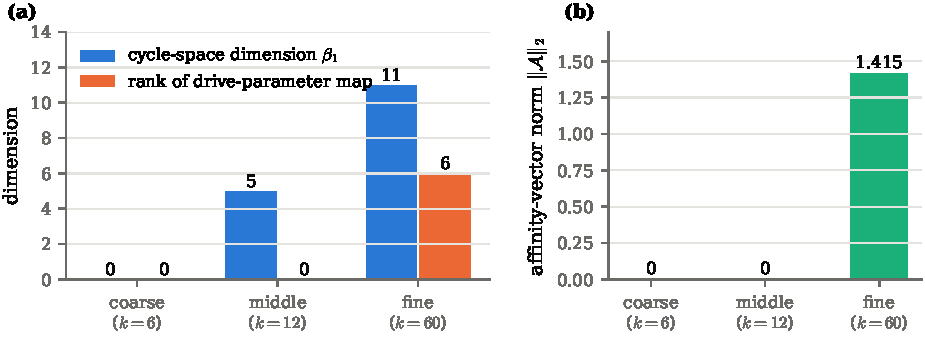
\includegraphics[width=\linewidth]{figures/fig_ladder.pdf}
\caption{Available versus active drive coordinates on the ladder chain. (a)~Cycle-space dimension \(\betaone\) of the lumped support graph and rank of the linear map from the six ring affinities \(A_1,\dots,A_6\) to cycle affinities. (b)~Euclidean norm of the cycle-affinity vector in the computed basis, which is basis-dependent and is shown for comparison within each level only. The half-ring level has five independent loops but no drive.}
\label{fig:ladder}
\end{figure}

\subsection{A ledger cost predicts better than a proxy}\label{sec:lab-proxy}

Is any low-dimensional penalty as good as a ledger-derived one? We build a ledger cost \(u^{\mathrm{led}}\) as in Section~\ref{sec:lab-price}, now with \(k=16\) random blocks, and take as ground truth the Gibbs kernel \(q^{\mathrm{true}}\) at the budget \(\cmin+0.35(c_0-\cmin)\). The proxy \(u^{\mathrm{prx}}\) rearranges the entries of each row of \(u^{\mathrm{led}}\) by a row-specific random permutation; the permutations are drawn once from a fixed seed and used for every sample. It therefore has exactly the same values in every row, attached to the wrong transitions.

For each of five samples we draw \(30\) training and \(5000\) test transitions per row and compare three models: row-wise empirical frequencies (clipped below \(10^{-12}\) and renormalized), and one-price Gibbs models fitted with \(u^{\mathrm{led}}\) and with \(u^{\mathrm{prx}}\). The price is fitted by maximizing the conditional-logit likelihood \(\ell(\lambda)=\sum_{ij}C_{ij}\log q^\lambda_{ij}\) \cite{mcfadden1974conditional}. This likelihood is concave, with curvature \(\sum_iN_i\Var_{q^\lambda_{i\cdot}}(u_{i\cdot})\), where \(N_i\) is the number of training transitions from row \(i\). The price is identifiable when some observed row has nonconstant cost. If some observed row has nonconstant cost but every observed transition already minimizes its row's cost, the likelihood keeps increasing and the fitted price is \(+\infty\). An optimum at the boundary \(\lambda=0\) can occur, and then the inverse curvature is not a symmetric confidence interval.

\paragraph{Prediction.} The ledger model has the lower held-out negative log-likelihood in every sample, with a mean of \(2.103\) per transition against \(2.773\) for the proxy and \(5.157\) for empirical frequencies (Figure~\ref{fig:proxy}). The empirical baseline does badly because \(30\) draws over \(16\) destinations leave many transitions unseen, which then receive probability near zero. The proxy model does no better than uniform guessing, whose loss is \(\log16\approx2.7726\). The direction of the gap is expected. Since the data come from \(q^{\mathrm{true}}\), any fixed kernel \(r\) has expected excess held-out loss per transition \(\sum_iw_i\,\KL(q^{\mathrm{true}}_{i\cdot}\|r_{i\cdot})\ge0\) over the truth, where \(w_i\) is the share of test transitions from row \(i\). This excess is strictly positive unless \(r\) agrees with the truth on every row with \(w_i>0\). A model family that contains the truth, as the ledger family does, can drive that excess toward zero as the training data grow. The proxy family contains the truth only if its permuted costs happen to induce the same Gibbs rows, which they do not here.

\paragraph{Prices.} The fitted ledger prices range from \(62.1\) to \(70.3\) (s.d.\ \(3.18\)), while the proxy prices range from \(0\) to \(1.67\) (s.d.\ \(0.55\)), with one sample at the boundary \(\lambda=0\). The proxy's smaller spread is not a sign of a better currency. Its fits stay near the uniform model, and prices attached to different cost coordinates do not share a scale. Prediction, not across-sample price variability, is the comparison this design supports.

\begin{figure}[tbp]
\centering
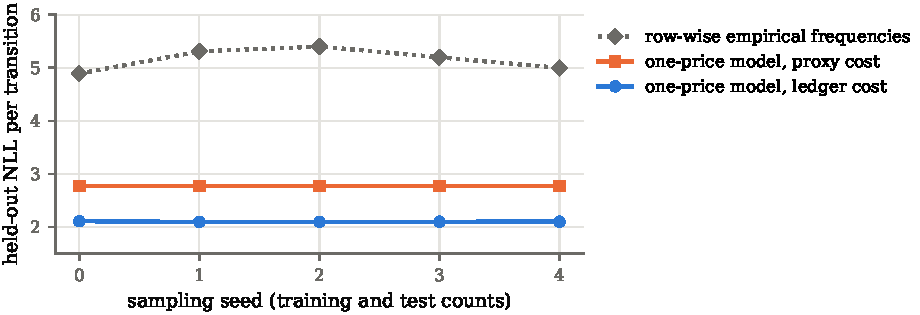
\includegraphics[width=\linewidth]{figures/fig_proxy.pdf}
\caption{Held-out negative log-likelihood per transition for five independent samples from a fixed design. The proxy cost has exactly the same values in each row as the ledger cost but attaches them to the wrong transitions; its fit is close to the uniform model, whose loss is \(\log 16\approx2.7726\).}
\label{fig:proxy}
\end{figure}

\subsection{Pricing exits buys object stability}\label{sec:lab-packaging}

Finally we connect the price to objecthood itself. Partition the states into blocks with \(f\), and let \(\pi\) be a stationary law of \(P\) with positive mass \(\pi(a)\) on every block \(a\). Packaging pushes a distribution forward to blocks and lifts it back with the stationary prototypes \(\nu_a=\pi(\cdot\mid a)\). For an integer number of steps \(\tau\ge0\),
\[
\mathcal B(\mu)=\sum_a\mu\big(f^{-1}(a)\big)\,\nu_a,\qquad
E_\tau(\mu)=\mathcal B(\mu P^\tau),\qquad
\delta(\mu)=\big\|E_\tau(E_\tau(\mu))-E_\tau(\mu)\big\|_1 .
\]
The map \(\mathcal B\) is stochastic and idempotent. The defect \(\delta\in[0,2]\) measures how much a packaged object moves when it is evolved and repackaged once more \cite{tsiokos2026sixbirds}.

\begin{theorem}[Packaging defect bound]\label{thm:packaging}
Let \(\varepsilon=\max_i\sum_{j:f(j)\ne f(i)}P_{ij}\) be the largest one-step exit probability from a block. Then for every probability law \(\mu\),
\[
\delta(\mu)\le\min(2,\,2\tau\varepsilon).
\]
\end{theorem}

The proof (Appendix~\ref{app:proofs}) uses stationarity: the mass a prototype loses from its block in one step equals the mass flowing into the block from outside, so one step moves \(\nu_a\) by at most \(2\varepsilon\) in \(\ell_1\) distance. This adds up to at most \(2\tau\varepsilon\) over \(\tau\) steps, and the bound extends to all lifted laws by convexity. The argument needs the stationary prototype; it is not claimed for uniform prototypes of a nonuniform block.

Now price the exits. Multiplying every inter-block transition by \(e^{-\lambda}\) and renormalizing gives \(P^{(\lambda)}\). If row \(i\) keeps mass \(r_i\) inside its block and sends \(s_i=1-r_i\) out, its exit probability becomes
\[
\varepsilon_i(\lambda)=\frac{s_i e^{-\lambda}}{r_i+s_ie^{-\lambda}}\le\frac{s_i}{r_i}\,e^{-\lambda}.
\]
When every \(r_i>0\), as in the module-ring chain, Theorem~\ref{thm:packaging} gives \(\delta\le2\tau\max_i(s_i/r_i)\,e^{-\lambda}\to0\). For a large enough exit price, every packaged object is therefore uniformly close to idempotent. The bound does not imply that the defect decreases monotonically in \(\lambda\) for every kernel family, because the prototypes change with \(\lambda\). If some row has \(r_i=0\), no vanishing-exit conclusion follows.

\paragraph{Experiment.} We take the module-ring chain with rings as blocks (\(k=6\)) and \(\tau=5\). The prices are calibrated with an auxiliary \(6\times6\) Gibbs problem whose cost is \(1\) for leaving a block and \(0\) for staying, with uniform row weights. Fifteen budgets between \(0.042\) and \(0.917\) give prices from \(4.74\) down to \(0\). The two budgets above \(c_0=5/6\) are slack. We report the defect at each block prototype; by linearity of \(E_\tau\), the largest of these is the worst defect over all lifted laws.

The mean defect over blocks falls from \(0.116\) at \(\lambda=0\) to \(0.00144\) at \(\lambda=4.74\), and the worst block falls from \(0.136\) to \(0.00173\) (Figure~\ref{fig:packaging}a). Every value lies below the bound \(2\tau\varepsilon_\lambda\), which falls from \(1.67\) to \(0.0174\), and the defect decreases along the whole sampled sweep.

The calibration budget should not be read as the substrate's spending. The auxiliary problem lives on a complete \(6\times6\) block graph, whereas the controlled chain can leave a ring only through its bridges. Its actual stationary exit rate, \(\sum_i\pi_\lambda(i)\sum_{j:f(j)\ne f(i)}P^{(\lambda)}_{ij}\), runs from \(0.0164\) down to \(1.4\times10^{-4}\), between about \(50\) and \(300\) times below the calibration cost (Figure~\ref{fig:packaging}b). The experiment thus demonstrates enforcement by a calibrated price, with actual spending measured separately.

\begin{figure}[tbp]
\centering
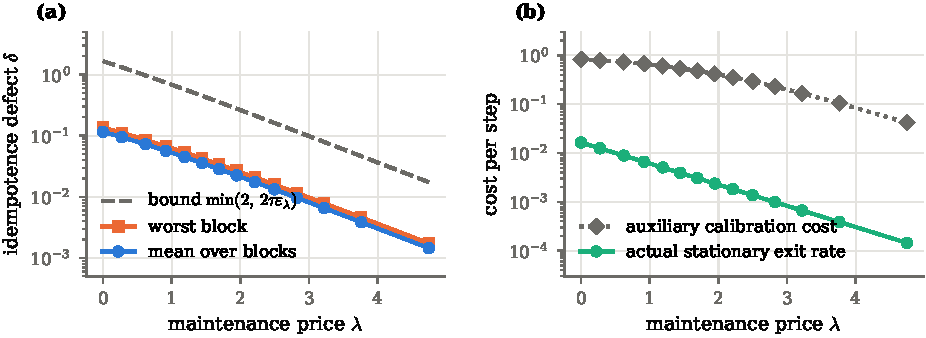
\includegraphics[width=\linewidth]{figures/fig_packaging.pdf}
\caption{Pricing block exits makes packaged objects nearly idempotent. (a)~Idempotence defect of the stationary block prototypes (mean and worst block) and the bound \(\min(2,2\tau\varepsilon_\lambda)\) of Theorem~\ref{thm:packaging}, with \(\tau=5\). (b)~The auxiliary calibration cost used to choose \(\lambda\), compared with the actual stationary exit rate of the controlled chain. Prices are calibrated, not inferred from spending.}
\label{fig:packaging}
\end{figure}

\FloatBarrier
